% answers.tex —— 2008 年·普通高等学校招生考试·上海卷·理科 · 参考答案与详细解析片段
% 由 tools/generate_projects.py 依来源总账自 2008/2008_数学真题_上海理_试题.md + 2008/2008_数学真题_上海理_解析正文.md + 2008/2008_数学真题_上海理_答案要点.md 生成，勿手改（改源 MD 后重跑）


\begin{gktip}
固定候选 PDF 仅含题面，无答案、解析和评分标准，原卷亦未标注分值；以下为非官方编者独立推导，官方答案字段为空。来源发布者、出版者、版次与官方身份均未核。
\end{gktip}

\begin{answer}
\gksolhead{1}{}

\textbf{题目}：

不等式 $|x-1|<1$ 的解集是\gkblank{}。

\Needspace{4\baselineskip}
\textbf{解析}

\Needspace{5\baselineskip}
计算如下：

\nopagebreak[4]
\[|x-1|<1\ \Longleftrightarrow\ 0<x<2.\]

\gkanswer{答案：$(0,2)$。}

\end{answer}
\begin{answer}
\gksolhead{2}{}

\textbf{题目}：

若集合 $A=\{x\mid x\leqslant2\}$，$B=\{x\mid x\geqslant a\}$ 满足 $A\cap B=\{2\}$，则实数 $a=$\gkblank{}。

\Needspace{4\baselineskip}
\textbf{解析}

$A\cap B=[a,2]$，要使它等于 $\{2\}$，需 $a=2$。

\gkanswer{答案：$2$。}

\end{answer}
\begin{answer}
\gksolhead{3}{}

\textbf{题目}：

若复数 $z$ 满足 $z=\mathrm i(2-z)$（$\mathrm i$ 是虚数单位），则 $z=$\gkblank{}。

\Needspace{4\baselineskip}
\textbf{解析}

\Needspace{5\baselineskip}
计算如下：

\nopagebreak[4]
\[z(1+\mathrm i)=2\mathrm i,\qquad z=\frac{2\mathrm i}{1+\mathrm i}=\mathrm i(1-\mathrm i)=1+\mathrm i.\]

\gkanswer{答案：$1+\mathrm i$。}

\end{answer}
\begin{answer}
\gksolhead{4}{}

\textbf{题目}：

若函数 $f(x)$ 的反函数为 $f^{-1}(x)=x^2$（$x>0$），则 $f(4)=$\gkblank{}。

\Needspace{4\baselineskip}
\textbf{解析}

$f^{-1}(x)=x^2$（$x>0$）的反函数为 $f(x)=\sqrt x$（$x>0$），故 $f(4)=2$。

\gkanswer{答案：$2$。}

\end{answer}
\begin{answer}
\gksolhead{5}{}

\textbf{题目}：

若向量 $\boldsymbol a$，$\boldsymbol b$ 满足 $|\boldsymbol a|=1$，$|\boldsymbol b|=2$，且 $\boldsymbol a$ 与 $\boldsymbol b$ 的夹角为 $\dfrac{\pi}3$，则 $|\boldsymbol a+\boldsymbol b|=$\gkblank{}。

\Needspace{4\baselineskip}
\textbf{解析}

\Needspace{5\baselineskip}
计算如下：

\nopagebreak[4]
\[|\boldsymbol a+\boldsymbol b|^2=1+4+2\times1\times2\cos\frac{\pi}3=7.\]

\gkanswer{答案：$\sqrt7$。}

\end{answer}
\begin{answer}
\gksolhead{6}{}

\textbf{题目}：

函数 $f(x)=\sqrt3\sin x+\sin\left(\dfrac{\pi}2+x\right)$ 的最大值是\gkblank{}。

\Needspace{4\baselineskip}
\textbf{解析}

\Needspace{5\baselineskip}
计算如下：

\nopagebreak[4]
\[f(x)=\sqrt3\sin x+\cos x=2\sin\left(x+\frac{\pi}6\right),\]

故最大值为 $2$。

\gkanswer{答案：$2$。}

\end{answer}
\begin{answer}
\gksolhead{7}{}

\textbf{题目}：

在平面直角坐标系中，从六个点 $A(0,0)$，$B(2,0)$，$C(1,1)$，$D(0,2)$，$E(2,2)$，$F(3,3)$ 中任取三个，这三点能构成三角形的概率是\gkblank{}。（结果用分数表示）

\Needspace{4\baselineskip}
\textbf{解析}

任取三点共 $\mathrm C_6^3=20$ 种。三点共线的情形：

$A(0,0)$，$C(1,1)$，$E(2,2)$，$F(3,3)$ 四点在直线 $y=x$ 上，任取三点共 $\mathrm C_4^3=4$ 种；另有 $B(2,0)$，$C(1,1)$，$D(0,2)$ 在直线 $y=-x+2$ 上，$1$ 种。

\Needspace{5\baselineskip}
共 $5$ 种共线，故概率为

\nopagebreak[4]
\[\frac{20-5}{20}=\frac34.\]

\gkanswer{答案：$\dfrac34$。}

\end{answer}
\begin{answer}
\gksolhead{8}{}

\textbf{题目}：

设函数 $f(x)$ 是定义在 $\mathbf R$ 上的奇函数。若当 $x\in(0,+\infty)$ 时，$f(x)=\lg x$，则满足 $f(x)>0$ 的 $x$ 的取值范围是\gkblank{}。

\Needspace{4\baselineskip}
\textbf{解析}

$x>0$ 时，$\lg x>0$ 给出 $x>1$。

$x<0$ 时，$f(x)=-f(-x)=-\lg(-x)>0$，即 $\lg(-x)<0$，故 $0<-x<1$，即 $-1<x<0$。

合得 $x\in(-1,0)\cup(1,+\infty)$。

\gkanswer{答案：$(-1,0)\cup(1,+\infty)$。}

\end{answer}
\begin{answer}
\gksolhead{9}{}

\textbf{题目}：

已知总体的各个体的值由小到大依次为 $2$，$3$，$3$，$7$，$a$，$b$，$12$，$13.7$，$18.3$，$20$，且总体的中位数为 $10.5$。若要使该总体的方差最小，则 $a$，$b$ 的取值分别是\gkblank{}。

\Needspace{4\baselineskip}
\textbf{解析}

\Needspace{5\baselineskip}
中位数 $\dfrac{a+b}2=10.5$，故 $a+b=21$。均值

\nopagebreak[4]
\[\bar x=\frac{79+21}{10}=10.\]

方差最小时 $a$，$b$ 尽量接近 $10$，结合 $a+b=21$、$7\leqslant a\leqslant b\leqslant12$，取 $a=10$，$b=11$。

\gkanswer{答案：$a=10$，$b=11$。}

\end{answer}
\begin{answer}
\gksolhead{10}{}

\textbf{题目}：

某海域内有一孤岛，岛四周的海平面（视为平面）上有一浅水区（含边界），其边界是长轴长为 $2a$，短轴长为 $2b$ 的椭圆。已知岛上甲、乙导航灯的海拔高度分别为 $h_1$，$h_2$，且两个导航灯在海平面上的投影恰好落在椭圆的两个焦点上，现有船只经过该海域（船只的大小忽略不计），在船上测得甲、乙导航灯的仰角分别为 $\theta_1$，$\theta_2$，那么船只已进入该浅水区的判别条件是\gkblank{}。

\Needspace{4\baselineskip}
\textbf{解析}

\Needspace{5\baselineskip}
设船在 $X$ 处，两导航灯在海平面上的投影为椭圆焦点 $F_1$，$F_2$，则

\nopagebreak[4]
\[\tan\theta_i=\frac{h_i}{|XF_i|}\ \Longrightarrow\ |XF_i|=h_i\cot\theta_i.\]

\Needspace{5\baselineskip}
船进入浅水区（含边界）等价于点 $X$ 在椭圆内或椭圆上，即

\nopagebreak[4]
\[|XF_1|+|XF_2|\leqslant2a,\]

\Needspace{5\baselineskip}
故判别条件为

\nopagebreak[4]
\[h_1\cot\theta_1+h_2\cot\theta_2\leqslant2a.\]

\gkanswer{答案：$h_1\cot\theta_1+h_2\cot\theta_2\leqslant2a$。}

\end{answer}
\begin{answer}
\gksolhead{11}{}

\textbf{题目}：

方程 $x^2+\sqrt2x-1=0$ 的解可视为函数 $y=x+\sqrt2$ 的图象与函数 $y=\dfrac1x$ 的图象交点的横坐标。若 $x^4+ax-4=0$ 的各个实根 $x_1$，$x_2$，$\cdots$，$x_k$（$k\leqslant4$）所对应的点 $\left(x_i,\dfrac4{x_i}\right)$（$i=1,2,\cdots,k$）均在直线 $y=x$ 的同侧，则实数 $a$ 的取值范围是\gkblank{}。

\Needspace{4\baselineskip}
\textbf{解析}

\Needspace{5\baselineskip}
点 $\left(x_i,\dfrac4{x_i}\right)$ 均在 $y=x$ 同侧，等价于 $\dfrac4{x_i}-x_i=\dfrac{4-x_i^2}{x_i}$ 对一切实根同号。该式在

\nopagebreak[4]
\[(0,2)\cup(-\infty,-2)\]

\Needspace{5\baselineskip}
上为正，在 $(2,+\infty)\cup(-2,0)$ 上为负。记

\nopagebreak[4]
\[h(x)=x^4+ax-4,\qquad h(0)=-4,\ h(2)=12+2a,\ h(-2)=12-2a.\]

若 $a<-6$：$h(2)<0$，$h(-2)>0$。$h'(x)=4x^3+a$ 只有一个实零点且为正，故 $h$ 恰有两个实根，分别在 $(-2,0)$ 与 $(2,+\infty)$，都属于“负”侧。

若 $a>6$：$h(2)>0$，$h(-2)<0$，同理恰有两个实根，分别在 $(0,2)$ 与 $(-\infty,-2)$，都属于“正”侧。

若 $-6<a<6$：$h(0)<0$ 而 $h(2)>0$，$h(-2)>0$，故在 $(0,2)$ 与 $(-2,0)$ 各有一根，两侧符号不同，不符。

\Needspace{5\baselineskip}
$a=\pm6$ 时根落在 $y=x$ 上，不符“同侧”。故

\nopagebreak[4]
\[a<-6\ \text{\text{或}}\ a>6.\]

\gkanswer{答案：$a<-6$ 或 $a>6$。}

\end{answer}
\begin{answer}
\gksolhead{12}{}

\textbf{题目}：

组合数 $\mathrm C_n^r$（$n>r\geqslant1$，$n$，$r\in\mathbf Z$）恒等于（　）

（A）$\dfrac{r+1}{n+1}\mathrm C_{n-1}^{r-1}$

（B）$(n+1)(r+1)\mathrm C_{n-1}^{r-1}$

（C）$nr\mathrm C_{n-1}^{r-1}$

（D）$\dfrac nr\mathrm C_{n-1}^{r-1}$

\Needspace{4\baselineskip}
\textbf{解析}

\Needspace{5\baselineskip}
计算如下：

\nopagebreak[4]
\[\mathrm C_n^r=\frac{n!}{r!(n-r)!}=\frac nr\cdot\frac{(n-1)!}{(r-1)!(n-r)!}=\frac nr\mathrm C_{n-1}^{r-1}.\]

\gkanswer{答案：D。}

\end{answer}
\begin{answer}
\gksolhead{13}{}

\textbf{题目}：

给定空间中的直线 $l$ 及平面 $\alpha$，条件“直线 $l$ 与平面 $\alpha$ 内无数条直线都垂直”是“直线 $l$ 与平面 $\alpha$ 垂直”的（　）

（A）充要条件

（B）充分非必要条件

（C）必要非充分条件

（D）既非充分又非必要条件

\Needspace{4\baselineskip}
\textbf{解析}

$l\perp\alpha$ 时 $l$ 垂直于 $\alpha$ 内所有直线，必垂直于无数条，必要性成立；反之只垂直于一组平行直线也满足“无数条”，未必垂直于 $\alpha$，充分性不成立。

\gkanswer{答案：C。}

\end{answer}
\begin{answer}
\gksolhead{14}{}

\textbf{题目}：

若数列 $\{a_n\}$ 是首项为 $1$，公比为 $a-\dfrac32$ 的无穷等比数列，且 $\{a_n\}$ 各项的和为 $a$，则 $a$ 的值是（　）

（A）$1$

（B）$2$

（C）$\dfrac12$

（D）$\dfrac54$

\Needspace{4\baselineskip}
\textbf{解析}

\Needspace{5\baselineskip}
计算如下：

\nopagebreak[4]
\[\frac1{1-\left(a-\frac32\right)}=a\ \Longrightarrow\ 2a^2-5a+2=0\ \Longrightarrow\ a=2\ \text{\text{或}}\ \frac12.\]

收敛要求 $\left|a-\dfrac32\right|<1$：$a=2$ 时公比 $\dfrac12$ 符合；$a=\dfrac12$ 时公比 $-1$ 不符合。故 $a=2$。

\gkanswer{答案：B。}

\end{answer}
\begin{answer}
\gksolhead{15}{}

\textbf{题目}：

如图，在平面直角坐标系中，$\Omega$ 是一个与 $x$ 轴的正半轴、$y$ 轴的正半轴分别相切于点 $C$、$D$ 的定圆所围成区域（含边界），$A$、$B$、$C$、$D$ 是该圆的四等分点。若点 $P(x,y)$、点 $P'(x',y')$ 满足 $x\leqslant x'$ 且 $y\geqslant y'$，则称 $P$ 优于 $P'$。如果 $\Omega$ 中的点 $Q$ 满足：不存在 $\Omega$ 中的其它点优于 $Q$，那么所有这样的点 $Q$ 组成的集合是劣弧（　）
\nopagebreak[4]
\begin{center}% 2008 年上海卷理科第 15 题：圆 Ω 与 x、y 轴正半轴分别切于 C、D，
%   A、B、C、D 为圆的四等分点（A 上、B 右、C 下、D 左）。
% 来源 PDF：gaokaomath-src/普通高考/2008/2008上海理.pdf
% SHA-256：df3f761eb2551cc795c0efb1c90c284a54b95265e327f21abb60aa0f4bdd86a2
% 原页：2008上海理.pdf 第 1 页（A3 三栏）第 2 栏，书页码 479。
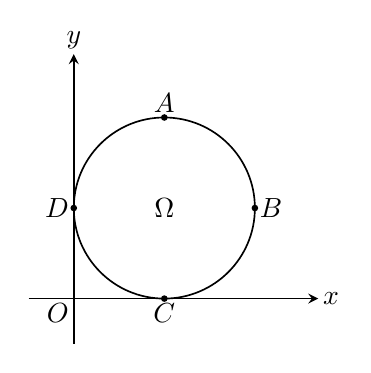
\begin{tikzpicture}[x=1.15cm, y=1.15cm, semithick,
  every node/.style={inner sep=1.5pt}]
  \draw[->,>=stealth] (-0.5,0) -- (2.7,0) node[right] {$x$};
  \draw[->,>=stealth] (0,-0.5) -- (0,2.7) node[above] {$y$};
  \node[below left] at (0,0) {$O$};
  \draw (1,1) circle (1);
  \node at (1,1) {$\Omega$};
  \fill (1,2) circle (1.2pt); \node[above] at (1,2) {$A$};
  \fill (2,1) circle (1.2pt); \node[right] at (2,1) {$B$};
  \fill (1,0) circle (1.2pt); \node[below] at (1,0) {$C$};
  \fill (0,1) circle (1.2pt); \node[left] at (0,1) {$D$};
\end{tikzpicture}
\end{center}
\nopagebreak[4]
（A）$\widehat{AB}$

（B）$\widehat{BC}$

（C）$\widehat{CD}$

（D）$\widehat{DA}$

\Needspace{4\baselineskip}
\textbf{解析}

圆心 $(r,r)$，$A(r,2r)$，$B(2r,r)$，$C(r,0)$，$D(0,r)$。对弧 $\widehat{DA}$ 上的点 $Q$，$\Omega$ 内横坐标不超过 $Q$ 的点都在 $Q$ 的右下方，不存在优于 $Q$ 的点；弧 $\widehat{AB}$、$\widehat{BC}$、$\widehat{CD}$ 上的点都可被更左更上的点优于。故所求为 $\widehat{DA}$。

\gkanswer{答案：D。}

\end{answer}
\begin{answer}
\gksolhead{16}{}

\textbf{题目}：

如图，在棱长为 $2$ 的正方体 $ABCD-A_1B_1C_1D_1$ 中，$E$ 是 $BC_1$ 的中点。求直线 $DE$ 与平面 $ABCD$ 所成角的大小。（结果用反三角函数表示）
\nopagebreak[4]
\begin{center}% 2008 年上海卷理科第 16 题：棱长 2 的正方体 ABCD-A1B1C1D1，E 为 BC1 的中点，
%   求直线 DE 与平面 ABCD 所成的角。
% 来源 PDF：gaokaomath-src/普通高考/2008/2008上海理.pdf
% SHA-256：df3f761eb2551cc795c0efb1c90c284a54b95265e327f21abb60aa0f4bdd86a2
% 原页：2008上海理.pdf 第 1 页（A3 三栏）第 2 栏，书页码 479。
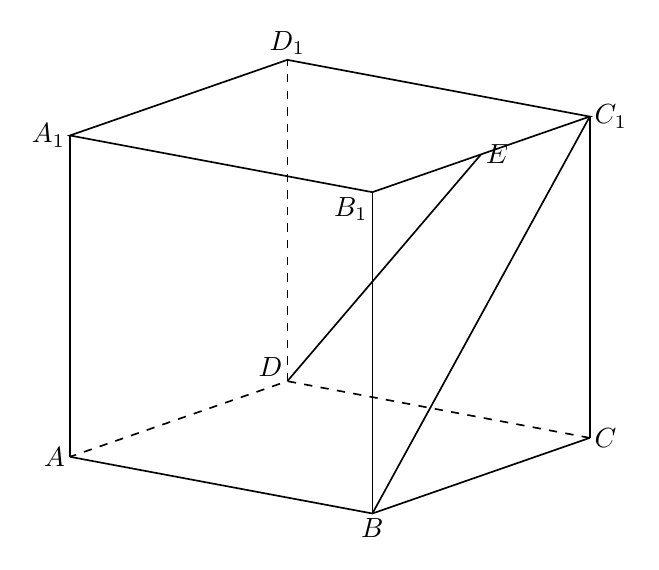
\begin{tikzpicture}[scale=1.2, semithick,
  every node/.style={inner sep=1.5pt}]
  \coordinate (A)  at (0.0,0.9);
  \coordinate (B)  at (3.2,0.3);
  \coordinate (C)  at (5.5,1.1);
  \coordinate (D)  at (2.3,1.7);
  \coordinate (A1) at (0.0,4.3);
  \coordinate (B1) at (3.2,3.7);
  \coordinate (C1) at (5.5,4.5);
  \coordinate (D1) at (2.3,5.1);
  \coordinate (E)  at (4.35,4.1);

  \draw (A) -- (B) -- (C);
  \draw[dashed] (C) -- (D) -- (A);
  \draw (A) -- (A1);
  \draw (B) -- (B1);
  \draw (C) -- (C1);
  \draw (D1) -- (A1) -- (B1) -- (C1) -- cycle;
  \draw[dashed] (D) -- (D1);

  \draw (D) -- (E);
  \draw (B) -- (C1);

  \node[left] at (A) {$A$};
  \node[below] at (B) {$B$};
  \node[right] at (C) {$C$};
  \node[above left] at (D) {$D$};
  \node[left] at (A1) {$A_1$};
  \node[below left] at (B1) {$B_1$};
  \node[right] at (C1) {$C_1$};
  \node[above] at (D1) {$D_1$};
  \node[right] at (E) {$E$};
\end{tikzpicture}
\end{center}
\nopagebreak[4]
\Needspace{4\baselineskip}
\textbf{解析}

\Needspace{5\baselineskip}
以 $A$ 为原点，$AB$，$AD$，$AA_1$ 为 $x$，$y$，$z$ 轴：

\nopagebreak[4]
\[D(0,2,0),\quad C_1(2,2,2),\quad E(2,1,1),\qquad \overrightarrow{DE}=(2,-1,1).\]

\Needspace{5\baselineskip}
平面 $ABCD$ 的法向量为 $(0,0,1)$，设线面角为 $\theta$：

\nopagebreak[4]
\[\sin\theta=\frac{1}{\sqrt6}=\frac{\sqrt6}6.\]

\gkanswer{答案：$\arcsin\dfrac{\sqrt6}6$。}

\end{answer}
\begin{answer}
\gksolhead{17}{}

\textbf{题目}：

如图，某住宅小区的平面图呈圆心角为 $120^\circ$ 的扇形 $AOB$。小区的两个出入口设置在点 $A$ 及点 $C$ 处，且小区里有一条平行于 $BO$ 的小路 $CD$。已知某人从 $C$ 沿 $CD$ 走到 $D$ 用了 $10$ 分钟，从 $D$ 沿 $DA$ 走到 $A$ 用了 $6$ 分钟。若此人步行的速度为每分钟 $50$ 米，求该扇形的半径 $OA$ 的长。（精确到 $1$ 米）
\nopagebreak[4]
\begin{center}% 2008 年上海卷理科第 17 题：圆心角 120° 的扇形 AOB，出入口在 A、C，
%   小路 CD∥BO，D 在 OA 上，CD=500 m，DA=300 m，求半径 OA。
% 来源 PDF：gaokaomath-src/普通高考/2008/2008上海理.pdf
% SHA-256：df3f761eb2551cc795c0efb1c90c284a54b95265e327f21abb60aa0f4bdd86a2
% 原页：2008上海理.pdf 第 1 页（A3 三栏）第 3 栏，书页码 479。
% 重绘依据：按 R=1 归一化，A 在 150°、B 在 30°，OD/R=145/445.45≈0.326，
%   CD/R=500/445.45≈1.123，C=(0.690,0.724) 落在单位圆上。
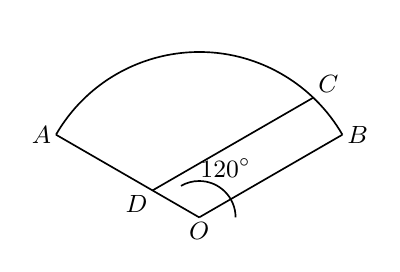
\begin{tikzpicture}[scale=2.1, semithick,
  every node/.style={inner sep=1.5pt}, font=\small]
  \coordinate (O) at (0,0);
  \coordinate (A) at (150:1);
  \coordinate (B) at (30:1);
  \coordinate (D) at (150:0.326);
  \coordinate (C) at (0.690,0.724);

  \draw (A) arc[start angle=150, end angle=30, radius=1];
  \draw (O) -- (A);
  \draw (O) -- (B);
  \draw (D) -- (C);

  \draw (0.22,0) arc[start angle=0, end angle=120, radius=0.22];
  \node at (0.16,0.30) {$120^\circ$};

  \node[left] at (A) {$A$};
  \node[right] at (B) {$B$};
  \node[above right] at (C) {$C$};
  \node[below left] at (D) {$D$};
  \node[below] at (O) {$O$};
\end{tikzpicture}
\end{center}
\nopagebreak[4]
\Needspace{4\baselineskip}
\textbf{解析}

\Needspace{5\baselineskip}
计算如下：

\nopagebreak[4]
\[CD=50\times10=500,\qquad DA=50\times6=300.\]

\Needspace{5\baselineskip}
设 $OA=R$，则 $OD=R-300$。以 $O$ 为原点、$OA$ 为 $x$ 轴，则 $OB$ 与 $OA$ 成 $120^\circ$：

\nopagebreak[4]
\[D(R-300,0),\qquad \overrightarrow{DC}\parallel\overrightarrow{OB},\ |\overrightarrow{DC}|=500.\]

\Needspace{5\baselineskip}
$OB$ 方向的单位向量为 $\left(-\dfrac12,\dfrac{\sqrt3}2\right)$，故

\nopagebreak[4]
\[C=\left(R-300-250,\ 250\sqrt3\right)=(R-550,250\sqrt3).\]

\Needspace{5\baselineskip}
$C$ 在圆上，$|OC|=R$：

\nopagebreak[4]
\[(R-550)^2+250^2\times3=R^2\ \Longrightarrow\ 1100R=490000,\]

\nopagebreak[4]
\[R=\frac{4900}{11}\approx445.45.\]

精确到 $1$ 米，$OA\approx445$ 米。

\gkanswer{答案：约 $445$ 米。}

\end{answer}
\begin{answer}
\gksolhead{18}{}

\textbf{题目}：

已知函数 $f(x)=\sin2x$，$g(x)=\cos\left(2x+\dfrac{\pi}6\right)$，直线 $x=t$（$t\in\mathbf R$）与函数 $f(x)$、$g(x)$ 的图象分别交于 $M$、$N$ 两点。

（1）当 $t=\dfrac{\pi}4$ 时，求 $|MN|$ 的值；

（2）求 $|MN|$ 在 $t\in\left[0,\dfrac{\pi}2\right]$ 时的最大值。

\Needspace{4\baselineskip}
\textbf{解析}

（1）$t=\dfrac{\pi}4$ 时 $f=1$，$g=\cos\dfrac{2\pi}3=-\dfrac12$，故 $|MN|=\dfrac32$。

\Needspace{5\baselineskip}
（2）

\nopagebreak[4]
\[f(t)-g(t)=\sin2t-\cos\left(2t+\frac{\pi}6\right)=\frac32\sin2t-\frac{\sqrt3}2\cos2t.\]

\Needspace{5\baselineskip}
再化为

\nopagebreak[4]
\[f(t)-g(t)=\sqrt3\sin\left(2t-\frac{\pi}6\right).\]

$t\in\left[0,\dfrac{\pi}2\right]$ 时 $2t-\dfrac{\pi}6\in\left[-\dfrac{\pi}6,\dfrac{5\pi}6\right]$，可取到 $1$，故 $|MN|_{\max}=\sqrt3$。

\gkanswer{答案：（1）$\dfrac32$；（2）$\sqrt3$。}

\end{answer}
\begin{answer}
\gksolhead{19}{}

\textbf{题目}：

已知函数 $f(x)=2^x-\dfrac1{2^{|x|}}$。

（1）若 $f(x)=2$，求 $x$ 的值；

（2）若 $2^tf(2t)+mf(t)\geqslant0$ 对于 $t\in[1,2]$ 恒成立，求实数 $m$ 的取值范围。

\Needspace{4\baselineskip}
\textbf{解析}

（1）$x\geqslant0$ 时 $2^x-2^{-x}=2$，得 $2^x=1+\sqrt2$，$x=\log_2(1+\sqrt2)$；$x<0$ 时左边为 $0$，无解。

\Needspace{5\baselineskip}
（2）$t\in[1,2]$ 时

\nopagebreak[4]
\[2^tf(2t)+mf(t)=2^{3t}-2^{-t}+m\left(2^t-2^{-t}\right).\]

\Needspace{5\baselineskip}
令 $u=2^t\in[2,4]$，两边乘 $u$ 得

\nopagebreak[4]
\[(u^2-1)(u^2+1+m)\geqslant0.\]

\Needspace{5\baselineskip}
$u^2-1>0$，故需 $u^2+1+m\geqslant0$ 对 $u\in[2,4]$ 恒成立：

\nopagebreak[4]
\[m\geqslant-\left(u^2+1\right)_{\max}=-5.\]

\gkanswer{答案：（1）$\log_2(1+\sqrt2)$；（2）$m\geqslant-5$。}

\end{answer}
\begin{answer}
\gksolhead{20}{}

\textbf{题目}：

设 $P(a,b)$（$b\neq0$）是平面直角坐标系 $xOy$ 中的点，$l$ 是经过原点与点 $(1,b)$ 的直线，记 $Q$ 是直线 $l$ 与抛物线 $x^2=2py$（$p\neq0$）的异于原点的交点。

（1）已知 $a=1$，$b=2$，$p=2$，求点 $Q$ 的坐标；

（2）已知点 $P(a,b)$（$ab\neq0$）在椭圆 $\dfrac{x^2}4+y^2=1$ 上，$p=\dfrac1{2ab}$，求证：点 $Q$ 落在双曲线 $4x^2-4y^2=1$ 上；

（3）已知动点 $P(a,b)$ 满足 $ab\neq0$，$p=\dfrac1{2ab}$，若点 $Q$ 始终落在一条关于 $x$ 轴对称的抛物线上，试问动点 $P$ 的轨迹落在哪种二次曲线上，并说明理由。

\Needspace{4\baselineskip}
\textbf{解析}

\Needspace{5\baselineskip}
（1）$p=2$ 时抛物线为 $x^2=4y$；$l$ 过原点与 $(1,2)$，故 $l:y=2x$。联立

\nopagebreak[4]
\[x^2=4\cdot2x=8x,\]

非零解 $x=8$，$y=16$，故 $Q(8,16)$。

\Needspace{5\baselineskip}
（2）$l:y=bx$。代入 $x^2=2py$：$x^2=2pbx$，非零解 $x=2pb$，故

\nopagebreak[4]
\[Q\left(2pb,\ 2pb^2\right).\]

\Needspace{5\baselineskip}
由 $p=\dfrac1{2ab}$ 得

\nopagebreak[4]
\[x_Q=2pb=\frac1a,\qquad y_Q=2pb^2=\frac ba.\]

\Needspace{5\baselineskip}
于是

\nopagebreak[4]
\[4x_Q^2-4y_Q^2=\frac{4}{a^2}-\frac{4b^2}{a^2}=\frac{4(1-b^2)}{a^2}.\]

$P$ 在椭圆上：$\dfrac{a^2}4+b^2=1$，即 $a^2=4(1-b^2)$，故上式等于 $1$，即 $Q$ 在双曲线 $4x^2-4y^2=1$ 上。

\Needspace{5\baselineskip}
（3）设 $Q(x,y)$ 恒在关于 $x$ 轴对称的抛物线 $y^2=2mx$（$m\neq0$）上。由（2），

\nopagebreak[4]
\[x=\frac1a,\qquad y=\frac ba,\]

\Needspace{5\baselineskip}
代入得

\nopagebreak[4]
\[\frac{b^2}{a^2}=2m\cdot\frac1a\ \Longrightarrow\ b^2=2ma.\]

故动点 $P(a,b)$ 的轨迹是抛物线 $y^2=2mx$（开口沿 $x$ 轴），即仍为抛物线。

\gkanswer{答案：（1）$(8,16)$；（2）证明见解析；（3）$P$ 的轨迹是抛物线（$y^2=2mx$ 型）。}

\end{answer}
\begin{answer}
\gksolhead{21}{}

\textbf{题目}：

已知以 $a_1$ 为首项的数列 $\{a_n\}$ 满足：$a_{n+1}=\begin{cases}a_n+c,&a_n<3,\\ \dfrac{a_n}d,&a_n\geqslant3.\end{cases}$

（1）当 $a_1=1$，$c=1$，$d=3$ 时，求数列 $\{a_n\}$ 的通项公式；

（2）当 $0<a_1<1$，$c=1$，$d=3$ 时，试用 $a_1$ 表示数列 $\{a_n\}$ 的前 $100$ 项的和 $S_{100}$；

（3）当 $0<a_1<\dfrac1m$（$m$ 是正整数），$c=\dfrac1m$，正整数 $d\geqslant3m$ 时，求证：数列 $a_2-\dfrac1m$，$a_{3m+2}-\dfrac1m$，$a_{6m+2}-\dfrac1m$，$a_{9m+2}-\dfrac1m$ 成等比数列当且仅当 $d=3m$。

\Needspace{4\baselineskip}
\textbf{解析}

\Needspace{5\baselineskip}
（1）$a_1=1$，$a_2=2$，$a_3=3$，$a_4=\dfrac33=1$，故

\nopagebreak[4]
\[a_1,a_2,a_3,a_4,\cdots=1,2,3,1,2,3,\cdots,\]

\Needspace{5\baselineskip}
即

\nopagebreak[4]
\[a_n=n-3\left\lfloor\frac{n-1}3\right\rfloor.\]

\Needspace{5\baselineskip}
（2）$0<a_1<1$，记 $t=a_1$。前四项

\nopagebreak[4]
\[a_1=t,\quad a_2=t+1,\quad a_3=t+2,\quad a_4=t+3,\]

$a_4\geqslant3$ 触发除法，$a_5=\dfrac{t+3}3=1+\dfrac t3$。

\Needspace{5\baselineskip}
此后每三项为

\nopagebreak[4]
\[u_k,\quad u_k+1,\quad u_k+2,\qquad u_k=1+\frac t{3^k},\]

第三项 $u_k+2\geqslant3$ 触发下一次除法，且 $u_{k+1}=\dfrac{u_k+2}3=1+\dfrac t{3^{k+1}}$。

\Needspace{5\baselineskip}
从 $a_5$ 到 $a_{100}$ 共 $96$ 项，恰为 $k=1,2,\cdots,32$ 的 $32$ 组三项。故

\nopagebreak[4]
\[S_{100}=(4t+6)+\sum_{k=1}^{32}\left(3u_k+3\right)
=4t+6+192+3t\sum_{k=1}^{32}\frac1{3^k}.\]

\nopagebreak[4]
\[\sum_{k=1}^{32}\frac1{3^k}=\frac12\left(1-3^{-32}\right),\]

\nopagebreak[4]
\[S_{100}=198+4t+\frac{3t}2\left(1-3^{-32}\right)=198+\frac t2\left(11-3^{-31}\right).\]

（3）记 $b_k=a_{3km+2}-\dfrac1m$（$k=0,1,2,3$），其中 $b_0=a_2-\dfrac1m=a_1$。

\Needspace{5\baselineskip}
由 $a_2=\dfrac1m+b_0$ 起，每次加 $\dfrac1m$；因 $b_0<\dfrac1m$，经 $3m-1$ 次达到 $\geqslant3$，除法后下一项为

\nopagebreak[4]
\[a_{3m+2}=\frac{b_0+3}{d},\]

\Needspace{5\baselineskip}
故

\nopagebreak[4]
\[b_1=\frac{b_0+3}{d}-\frac1m=\frac{b_0+3-\frac dm}{d}.\]

\Needspace{5\baselineskip}
一般地，$b_k>\dfrac1m$（$k\geqslant1$），同样经 $3m-1$ 次达到 $\geqslant3$，得递推

\nopagebreak[4]
\[b_{k+1}=\frac{b_k+3-\frac dm}{d}.\]

\Needspace{5\baselineskip}
若 $d=3m$，则

\nopagebreak[4]
\[b_{k+1}=\frac{b_k}{3m},\]

故 $b_0,b_1,b_2,b_3$ 成公比为 $\dfrac1{3m}$ 的等比数列。

\Needspace{5\baselineskip}
若 $d>3m$，记 $\alpha=\dfrac1d$，$\gamma=\dfrac{3-\frac dm}{d}<0$，则 $b_{k+1}=\alpha b_k+\gamma$，其不动点

\nopagebreak[4]
\[\beta=\frac{\gamma}{1-\alpha}<0.\]

\Needspace{5\baselineskip}
若 $b_0,b_1,b_2$ 成等比，则 $b_1^2=b_0b_2$，代入 $b_{k+1}=\alpha b_k+\gamma$ 得

\nopagebreak[4]
\[\gamma\left[(\alpha-1)b_0+\gamma\right]=0.\]

$\gamma\neq0$，故 $b_0=\beta<0$，与 $b_0=a_1>0$ 矛盾。故此时不成等比数列。

综上，所给四项成等比数列当且仅当 $d=3m$。

\gkanswer{答案：（1）$a_n$ 以 $1,2,3$ 循环；（2）$S_{100}=198+\dfrac{a_1}2\left(11-3^{-31}\right)$；（3）证明见解析。}

\end{answer}